%{{{
\documentclass{beamer}
\usetheme{ensam}
\usepackage{pgfplots}
\usepackage{subcaption}
\usepackage{acronym}
\usepackage{tikz}
\usetikzlibrary{calc}
\usepackage{amsmath}
\usepackage {algorithmic}
\usepackage{algorithm}
\usepackage{eqparbox}
\usepackage[font=scriptsize]{caption}
\usetikzlibrary{bayesnet,positioning,calc}
\tikzstyle{obs} = [latent,fill=lightBlue]
\tikzstyle{default}=[draw=sexyRed,thick,rounded corners,text width=0.5in,font=\scriptsize,align=center]
\usepgfplotslibrary{colorbrewer}
\definecolor{ForestGreen}{RGB}{34,139,34}
\newcommand{\comment}[1]{\textcolor{ForestGreen}{#1}}
% \newcommand{\P}{\mathbf{P}}
%algorithmic comment
\renewcommand\algorithmiccomment[1]{%
  \hfill\comment{\#\scriptsize\eqparbox{COMMENT}{#1}}%
}
\renewcommand{\algorithmicrequire}{\textbf{Input:}}
\renewcommand{\algorithmicensure}{\textbf{Output:}}
\title{Conditionnements}
\author{\underline{A.Belcaid}}
\institute{\small ENSA-Safi} 

%tikz bayesian theme
\usetikzlibrary{bayesnet,positioning,calc}
\tikzstyle{obs} = [latent,fill=lightBlue]
\tikzstyle{default}=[draw=sexyRed,thick,rounded corners,text width=0.5in,font=\scriptsize,align=center]
\DeclareMathOperator{\argmin}{argmin}

\pgfplotsset{every tick label/.append style={font=\tiny}}



%acronyms
\acrodef{MRF}{Markov Random Fields}
\acrodef{GNC}{Graduation nonconvexity}


% add bibliography
\usepackage[style=authoryear]{biblatex}
\renewcommand*{\nameyeardelim}{\addcomma\addspace}
\addbibresource{bibliography}
%}}}

\begin{document}
\maketitle

\begin{frame}
\tableofcontents
\end{frame}

% Introduction {{{ %
% Expliquer la situation de conditionement {{{ %
\begin{frame}[<+->]
    \frametitle{Introduction}
\scriptsize Les \alert{\textbf{probabilités conditionnelles}}  nous permet de
raisonner dans des conditions avec des \textbf{informations partielles}.\\[8pt]

\begin{enumerate}
    \scriptsize
    \item Dans une expérience avec plusieurs lancés de dé, On vous dit que la
        somme des lancés est $\mathbf{9}$. Quelle est la probabilité que le
        premier lancé est un $\mathbf{6}$.\\[8pt]
    \item Dans un jeu de devinette de mots, la première lettre est un
        \alert{\textbf{T}}. Quelle est la probabilité que la deuxième soit un
        \alert{\textbf{H}}?\\[8pt]
    \item Quelle est la probabilité qu'un patient est \alert{\textbf{malade}},
        étant donne que son test est \textbf{négatif}.\\[8pt]
    \item Un point s'affiche dans un radar d'observation, Quelle est la
        probabilité qu'elle correspond à un avion?
\end{enumerate}
\end{frame}
% }}} Expliquer la situation de conditionement %
% Utilites {{{ %
\begin{frame}[<+->]
    \frametitle{Conditionnement}
    
    \begin{enumerate}
        \item \alert{\textbf{Conditionnement}}:
            \begin{itemize}
                \item Modèle \structure{\textbf{révisé}} avec une nouvelle
                    information.\\[8pt]
                \item Un outil crucial pour \textbf{diviser pour régner}.\\[8pt]

            \end{itemize}
        \item \alert{\textbf{Indépendance}} 
    \end{enumerate}
\end{frame}
% }}} Utilites %

% }}} Introduction %
% Definition {{{ %
\section{Conditionnement}

\begin{frame}[t]
    \frametitle{Idée de conditionnement}
    \begin{columns}
        \begin{column}{0.5\textwidth}
\only<1->
{
        \centering
        \textbf{Idée} de Conditionnement.\\
        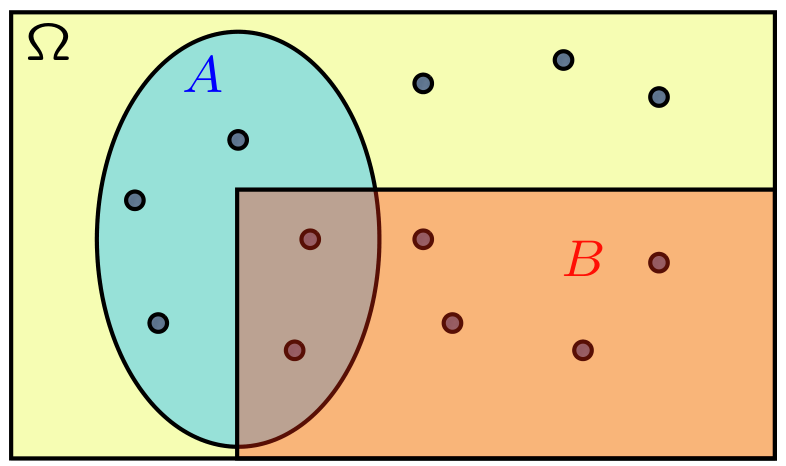
\includegraphics[width=0.8\textwidth]{./cond_first_example_1_1.png}

        $$
        \scriptsize
        \mathbf{P}(\structure{A}) =  \frac{5}{12}\quad \mathbf{P}(\alert{B}) =  \frac{6}{12}
        $$
}

\only<3->
{
        \centering
        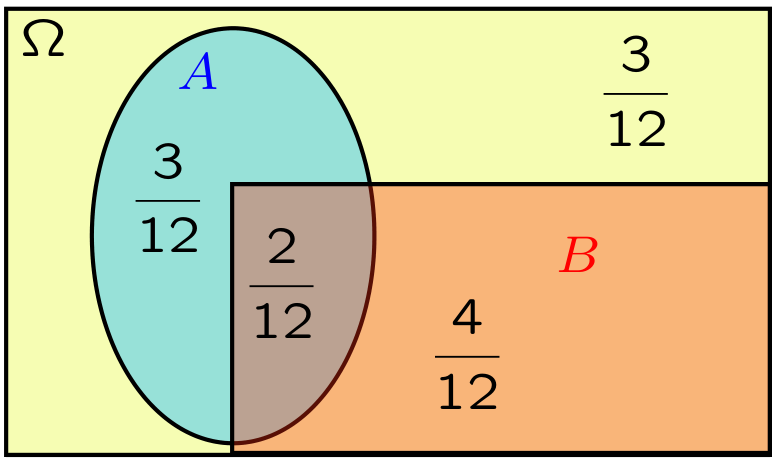
\includegraphics[width=0.8\textwidth]{./cond_first_example_1_3.png}

}
        \end{column}
        \begin{column}{0.5\textwidth}
            
\only<2->
{
        \centering
        \textbf{Évènement} $B$ est réalisé.\\
        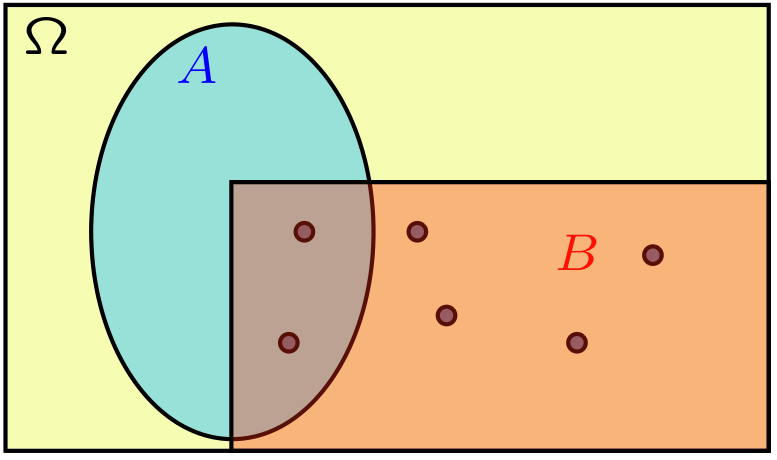
\includegraphics[width=0.8\textwidth]{./cond_first_example_1_2.png}

        $$
        \scriptsize
        \mathbf{P}(\structure{A} | \alert{B}) =  \frac{2}{6}\quad
        \mathbf{P}(\alert{B} | \alert{B} ) =  1
        $$
}

\only<4->
{
        \centering
        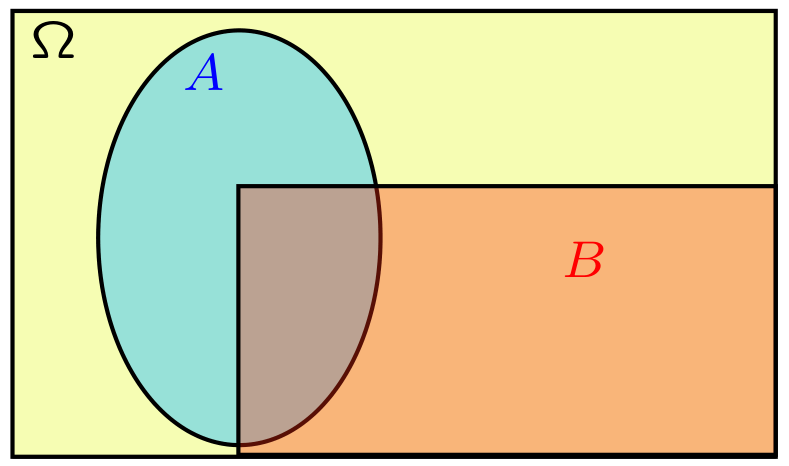
\includegraphics[width=0.8\textwidth]{./cond_first_example_1_4.png}

}
        \end{column}
    \end{columns}
    
\end{frame}
% }}} Definition %
% Definition conditioning {{{ %
\begin{frame}[t]
    \frametitle{Définition Conditionnement}
    \begin{center}
    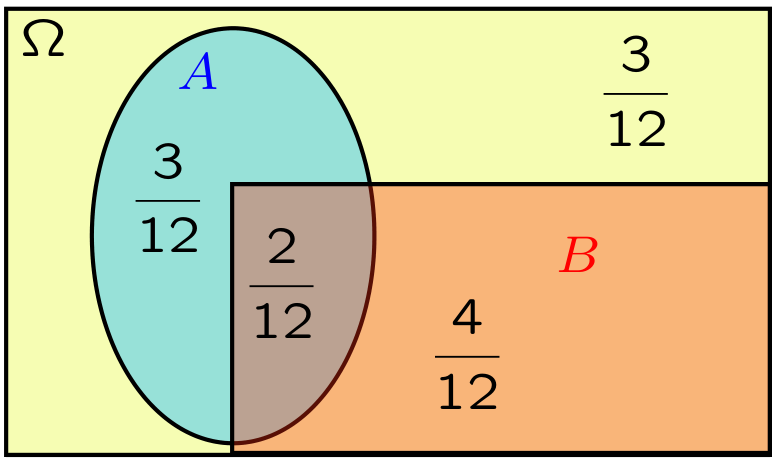
\includegraphics[width=0.4\textwidth]{./cond_first_example_1_3.png}
    \end{center}
    
    \pause
    \begin{itemize}
        \item $\mathbf{P}(A | B) =$ "\scriptsize probabilité A sachant B"
    \end{itemize}
    \begin{block}{Définition}
       \begin{equation}
          \mathbf{P}(A\;|\; B) = \dfrac{\mathbf{P}(A\cap B)}{\mathbf{P}(B)}
       \end{equation} 
    \end{block}
    \begin{itemize}
        \item Cette définition ne peut avoir sens que si $\mathbf{P}(B) > 0 $.
    \end{itemize}
\end{frame}
% }}} Definition conditioning %
% Exemple lance du de {{{ %

\begin{frame}[t]
    \frametitle{Exemple: Lance de deux dé}
   \begin{columns}
       \begin{column}{0.5\textwidth}
          \only<1->
          {


            \begin{center}
            \begin{tikzpicture}[scale=.8, transform shape]
                
                \draw[thick] (0,0) grid (4,4);
                \foreach \x/\y in {0.5/1, 1.5/2, 2.5/3, 3.5/4}
                {
                    \node at (\x,-.2) {\y};
                    \node at (-.2,\x) {\y};
                }
                \node at (2,-1) {\scriptsize lancé X};
                \node[rotate = 90] at (-1,2) {\scriptsize lancé Y};
                \only<3->{
                    \draw[fill,sexyRed, opacity=0.4] (1,1) rectangle(4,2);
                    \draw[fill,sexyRed, opacity=0.4] (1,1) rectangle(2,4);
                }

                \only<7->{
                    \draw[fill,blue, opacity=0.5] (2,0) rectangle(3,3);
                    \draw[fill,blue, opacity=0.5] (0,2) rectangle (3,3);
                }
            \end{tikzpicture}
            \end{center}
          }
       \end{column}
       \begin{column}{0.5\textwidth}
          \begin{itemize}
              \scriptsize
              \item<2-> Soit \alert{\textbf{B}} l'évènement: $\min(X, Y) =
                  2$.\\[0.5cm]
            
              \item<4-> Soit l'évènement  $M = \max(X,Y)$.
                  \vspace*{1cm}
                  \begin{itemize}
                      \item<5-> 
                          $$
                          P(M = 0   | B) = 
                          $$
                          \vspace*{1cm}
                      \item <6->
                          $$
                          P(M= 3 | B) = 
                          $$
                  \end{itemize}
          \end{itemize} 
       \end{column}
   \end{columns} 
\end{frame}
% }}} Exemple lance du de %
% Exercice {{{ %
\begin{frame}[t]
    \frametitle{Conditionnement : Mini Exercice}
    \begin{block}{Exemple}
        \small
        On considère  l'espace des probabilités qui consiste de l'unité $\Omega
        = [0,1]^2$. On considère un loi \textbf{uniforme} de probabilité qui
        donne la probabilité de chaque évènement par sa \textbf{surface}.\\[4pt]

        \begin{itemize}
            \item On considère l'évènement $B=\left\{(x,y)\;|\; y \leq x\right\}$
            \item Soit l'évènement $A= \left\{(x,y)\;|\; x \leq
                \frac{1}{2}\right\}$
        \end{itemize}
    \end{block}
    Calculer 
    $$
    P(A\;|\;B) = 
    $$
\end{frame}
% }}} Exercice %
% axioms conditional probability {{{ %
\begin{frame}[t]
    \frametitle{Axiomes probabilité conditionelle}
    
    \begin{columns}
        \begin{column}{0.5\textwidth}
           \begin{enumerate}
               \small
               \item<1->  $P(A\;|\;B) \geq 0$\\[8pt]
               \item<2-> $P(\Omega\;|\;B) = \frac{P\left(\Omega \cap
                   B\right)}{P(B)} = 1$\\[8pt]
               \item<3-> $P(B\;|\;B) = \frac{P\left(B \cap B\right)}{P(B)} =
                   1$\\[8pt]
               \item<4-> Si $A\cap C = \emptyset$ alors 
                   $$
                   P( A \cup C\;|\; B) = P(A\;|\; B) + P(A\;|\; B)
                   $$

            
           \end{enumerate} 
        \end{column}
        \begin{column}{0.5\textwidth}
           \only<4->
           {
    \centering
    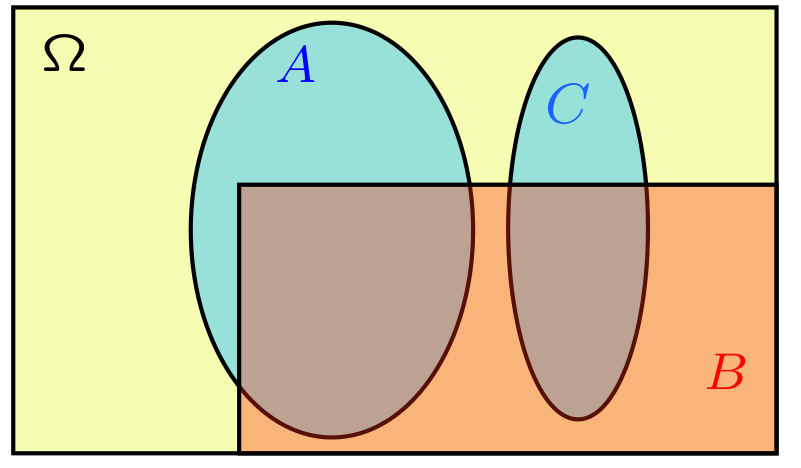
\includegraphics[width=0.8\textwidth]{./cond_axioms.png}
           }
        \end{column}
    \end{columns}
    \only<5->{
    \begin{block}{Important}
        \scriptsize
       Puisque ces axiomes sont vrais, toutes les formules dérivées en
       utilisant ces axiomes, reste \alert{\textbf{valide}}  pour les
       probabilités conditionnelles.
    \end{block}}
\end{frame}
% }}} axioms conditional probability %
% Modele base sur un conditionement {{{ %
\begin{frame}[t]
    \frametitle{Modèle base sur Conditionnement}
   \begin{columns}
       \begin{column}{0.4\textwidth}
           
        \begin{itemize}
            \scriptsize
            \item<1-> Évènement \structure{\textbf{A}}: Un avion vole dans l'air
            \item<4-> Évènement \alert{\textbf{B}}: On détecte l'avion dans le
                radar.\\[12pt]
            \item<9-> $P(A\cap B)$:\\[15pt]
            \item<10-> $P(B)$:\\[15pt]
            \item <11-> $P(A\;|\; B)$!!
        \end{itemize}
       \end{column}
       \begin{column}{0.6\textwidth}
           
           \only<10->
           {
               \begin{block}{}
                   
                   \scriptsize
                   \begin{equation*}
                       P(A\;|\; B) = \frac{ P(A \cap B)}{P(B)} \quad  P(B\;|\; A)
                       = \frac{P(A\cap B)}{P(A)}
                   \end{equation*}
               \end{block}
           }
           \vspace*{1cm}
           \begin{center}
           \begin{tikzpicture}[yscale=.8, transform shape]
               
               \only<2->
               {
                \draw[thick] (0,0) -- (2,1)node[label=above:{\small$A$}]{};
                \draw[thick] (0,0) -- (2,-1)node[label=below:{\small$A^c$}]{};
               }

               \only<3->{
                \node at (0, .6) {\scriptsize $P(A) = 0.05$};
                \node at (0, -.6) {\scriptsize $P(A^c) = 0.95$};
            }

            \only<5->
            {
                \draw[thick] (2,1) -- (4,1.5)node[label=right:{\small$A\cap B$}]{};
                \draw[thick] (2,1) -- (4,.5)node[label=right:{\small$A\cap B^c$}]{};
                \draw[thick] (2,-1) -- (4,-.5)node[label=right:{\small$A^c\cap B$}]{};
                \draw[thick] (2,-1) -- (4,-1.5)node[label=right:{\small$A^c\cap B^c$}]{};
            }
            \only<6->
            {
                \node (P) at (2.6,1.4) {\small$0.99$};
                \node at (2.6,0.6) {\small$0.01$};
            }
            \only<7->
            {
                \node (Pc) at (1.2,2.2) {\small\alert{$P(B \; |\; A)$}};
                \path[draw,->,>=latex] (Pc) -- (P);
            }

            \only<8->
            {
                \node  at (2.6,-0.4) {\small$0.10$};
                \node at (2.6,-1.6) {\small$0.90$};
            }
           \end{tikzpicture}
           \end{center}
       \end{column}
   \end{columns} 
\end{frame}
% }}} Modele base sur un conditionement %
% Rege de multiplication {{{ %
\begin{frame}[t]
    \frametitle{Règle de multiplication}
   \begin{columns}
       \begin{column}{0.4\textwidth}
          \scriptsize 
           \begin{equation*}
               P(A\;|\;B)  = \frac{ P(A\cap B)}{ P(B)}
           \end{equation*}
           \only<2->
           {

               \begin{eqnarray*}
                   P(A\cap B) & = & P(B)\;P(A\;|\;B) \\
                              & = & P(A)\;P(B\;|\; A)
               \end{eqnarray*}
           }
           \only<4->
           {
               \begin{equation*}
                   P\left(\structure{A^c}\cap \alert{B \cap C^c}\right)=
               \end{equation*}
           }
       \end{column}
       \begin{column}{0.6\textwidth}
           
           \only<3->
           {
                   \centering
                   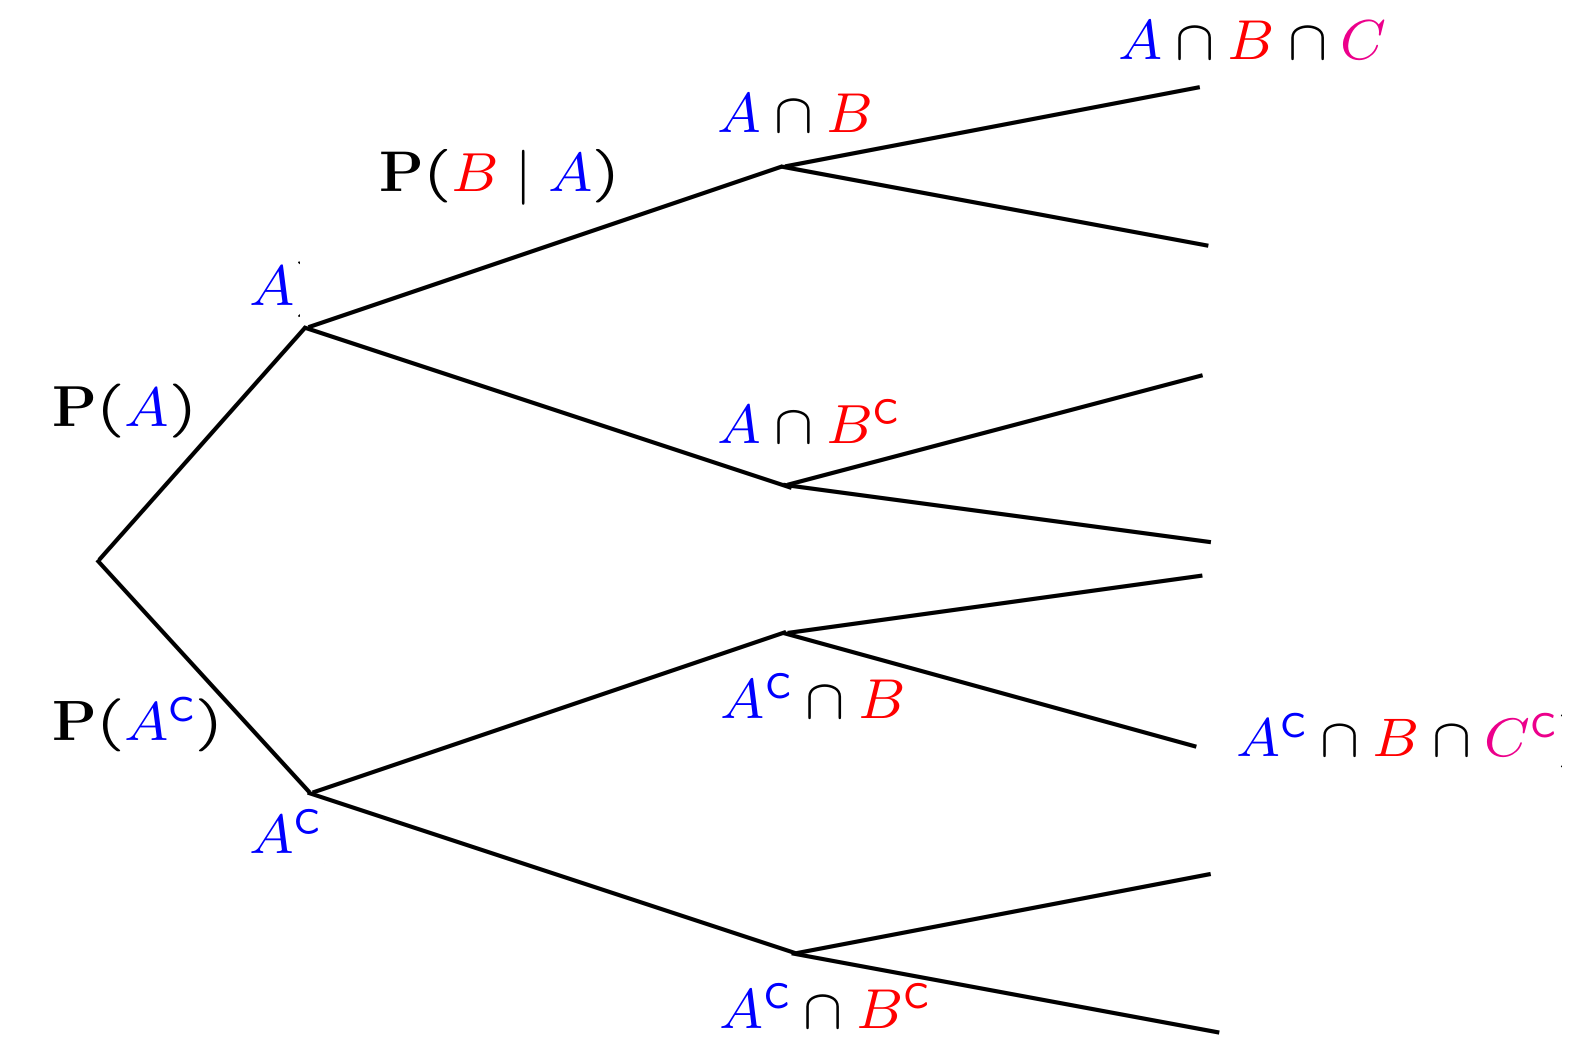
\includegraphics[width=0.8\textwidth, height=5cm]{./tree_event_multiplication.png}
           }
       \end{column}
   \end{columns} 

   \vspace*{1cm}
       \only<4->
       {
           \scriptsize
           \begin{equation*}
               \scriptsize
               P(A_1\cap A_2\cap\ldots A_n) = P(A_1)\prod_{i=2}^n P(A_i\;|\;
               A_1\cap A_2\cap\ldots\cap A_{i-1})
           \end{equation*}
       }

\end{frame}
% }}} Rege de multiplication %
% Mini Exercice {{{ %
\begin{frame}[<+->]
    \frametitle{Pratique règle multiplication}
   \begin{itemize}
       \small
       \item Est ce que les formules suivantes sont Correctes:\\[4pt]
           \begin{itemize}
               \scriptsize
               \item $P(A\cap B \cap C^c)  = P(A\cap B) P(C^c\;|A\cap B)$\\[12pt]
               \item $P(A\cap B \cap C^c)  = P(A) P(C^c\;|A) P(B\;|\;A\cap
                   C^c)$\\[12pt]
               \item $P(A\cap B\cap C^c) = P(A) P(C^c\cap A|A)P(B|A\cap
                   C^c)$\\[12pt]
               \item $P(A\cap B|C) = P(A|C)P(B|A\cap C)$
           \end{itemize}
   \end{itemize}  
\end{frame}
% }}} Mini Exercice %
% Formule de probabilité totale {{{ %
\begin{frame}[t]
    \frametitle{Formule de probabilité totale}
   \begin{columns}
       \begin{column}{0.4\textwidth}
           \only<1->
           {
                   \centering
                   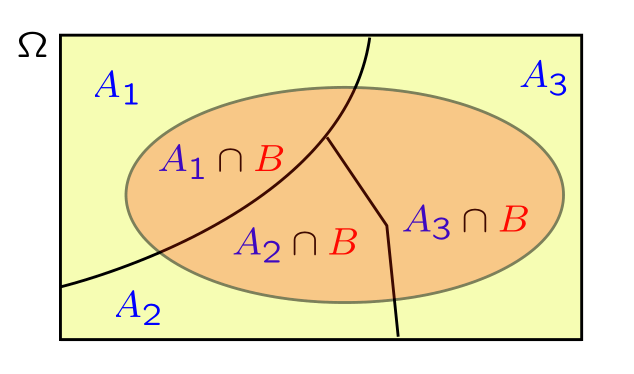
\includegraphics[width=0.9\textwidth]{./form_total_probablity.png}
               }
        \only<2->
        {
                \centering
                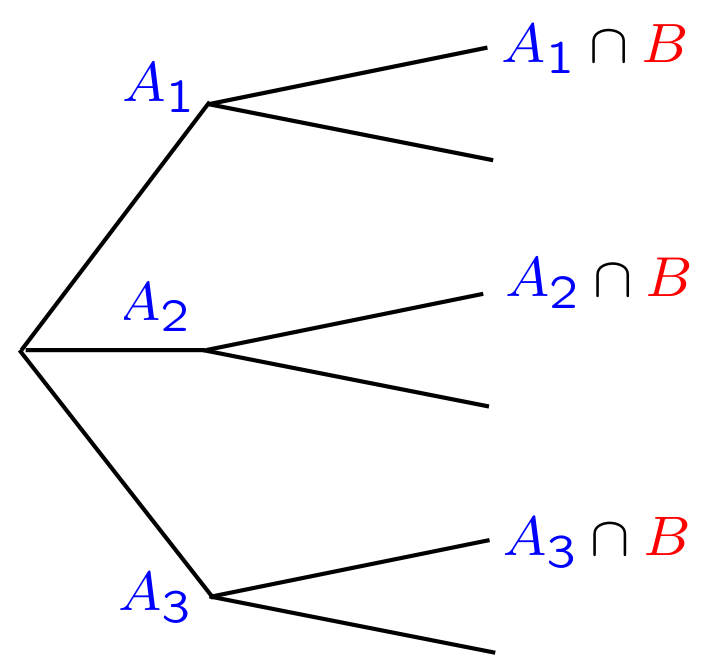
\includegraphics[width=0.8\textwidth]{./total_probability_tree.png}
        }
       \end{column}
       \begin{column}{0.6\textwidth}
           \begin{itemize}
               \scriptsize
               \item<1-> On possède une partition $\structure{A_1,A_2,A_3}$ de
                   l'ensemble $\Omega$. \\[8pt]
               \item<1-> On a $P(A_i)$ pour chaque $i$. 
               \item<3-> On possède $P(B \;|\; A_i)$ pour chaque $i$.
           \end{itemize}

           \only<4>
           {
               $$
               P(B)?
               $$
           }

           \only<5->
           {
               \scriptsize
               \begin{eqnarray*}
                   P(B) = P(B \cap A_1) + P(B \cap A_2) + P(B \cap A_3)
               \end{eqnarray*}
           }
           \only<6->
           {
               \begin{block}{Formule de probabilité totale.}
                   
                   \small
                   $$
                   P(B) = \sum_{i} P(A_i) P(B\;|\;A_i)
                   $$
               \end{block}
           }
       \end{column}

   \end{columns} 
\end{frame}
% }}} Formule de probabilité totale %
% Regle de Bayes {{{ %
\begin{frame}[t]
    \frametitle{Règle de Bayes}
    
   \begin{columns}
       \begin{column}{0.4\textwidth}
           \only<1->
           {
                   \centering
                   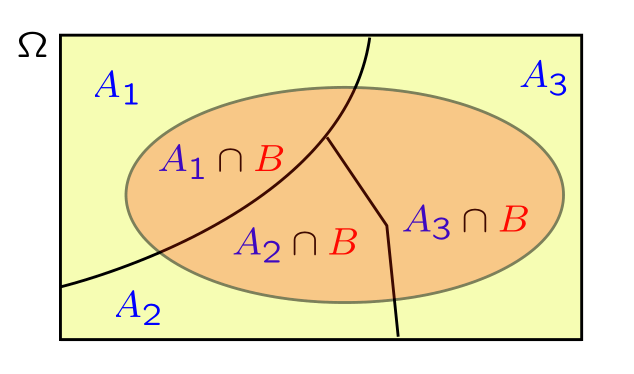
\includegraphics[width=0.9\textwidth]{./form_total_probablity.png}
               }
        \only<2->
        {
                \centering
                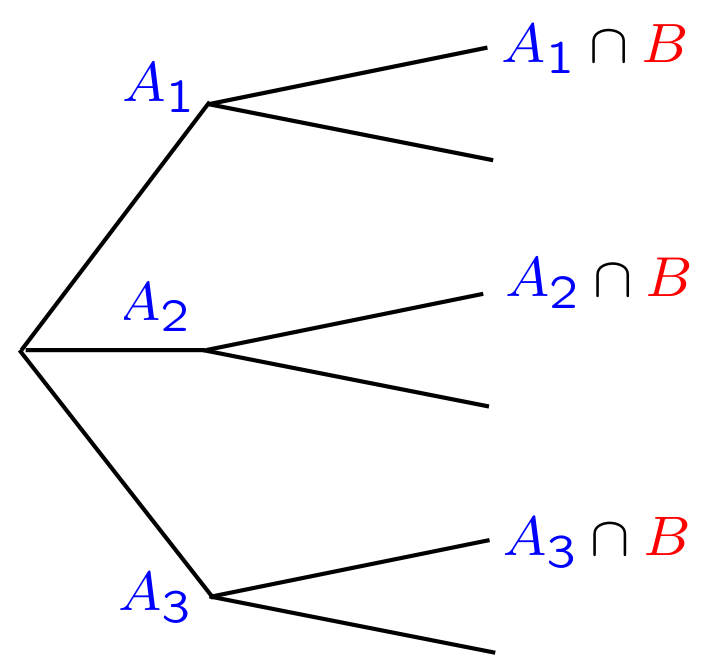
\includegraphics[width=0.8\textwidth]{./total_probability_tree.png}
        }
       \end{column}
       \begin{column}{0.6\textwidth}
           \begin{itemize}
               \scriptsize
               \item<1-> On possède une partition $\structure{A_1,A_2,A_3}$ de
                   l'ensemble $\Omega$. \\[8pt]
               \item<1-> On a $P(A_i)$ pour chaque $i$. \alert{\textbf{Croyances
                   a priori}} 
               \item<3-> On possède $P(B \;|\; A_i)$ pour chaque $i$.
                   \alert{\textbf{Croyances révisées}} 
           \end{itemize}

           \only<4>
           {
               $$
               P(\alert{A_i}\;|\; \structure{B})?
               $$
           }

           \only<5->
           {
               \scriptsize
               \begin{eqnarray*}
                   P(A_i\;|\;B) = \frac{ P(A_i \cap B)}{P(B)} 
               \end{eqnarray*}
           }
           \only<6->
           {
               \begin{block}{Formule de Bayes.}
                   
                   \small
                   $$
                   P(A_i\;|\; B) = \frac{P(A_i) P(B\;|\;A_i)}{P(B)} 
                   $$
               \end{block}
           }
       \end{column}

   \end{columns} 
\end{frame}
% }}} Regle de Bayes %
\end{document}
